\section{Methodology}
\label{sec:methodology}
% Focus on what you add to the existing method. Explain what you will do and why (and how). Do not forget to characterize your research design. There should be a sub-section on the evaluation. 
%For DS students, this normally means using manually labelled or ground truth data. 
% Write about your methodology here. Focus on your own contribution. Indicate exactly how you will assess your work in terms of evaluation.
% It is possible to use a separate section for the Experimental Setup, which then focuses on all settings used in your experiments. It also possible to address the settings in a sub-section under Methodology. 

The goal of the study is to understand the characteristics of storefront signage in relation to gentrification, via learning the font types, colors, and semantic present. The approach that this study takes comprises of multiple models: scene-text detection, scene-text recognition, color histogram, font recognition, word embedding, and gradient boosting. This is because the state-of-the-art is that there has not been a model that takes an interest in analyzing scene-text in a comprehensive manner - much of the focus is on detecting and recognizing text in the wild with better accuracy. Elements such as fonts and colors are only of interest in the domain of graphic design. Therefore, this research serves as a pilot case in utilizing these individual models for feature extraction via transfer learning, and subsequently test these features by using them to classify gentrified/non-gentrified storefronts.

The data pipeline is visualized in Figure \ref{fig:pipeline}.

\begin{figure*}[]
    \centering
    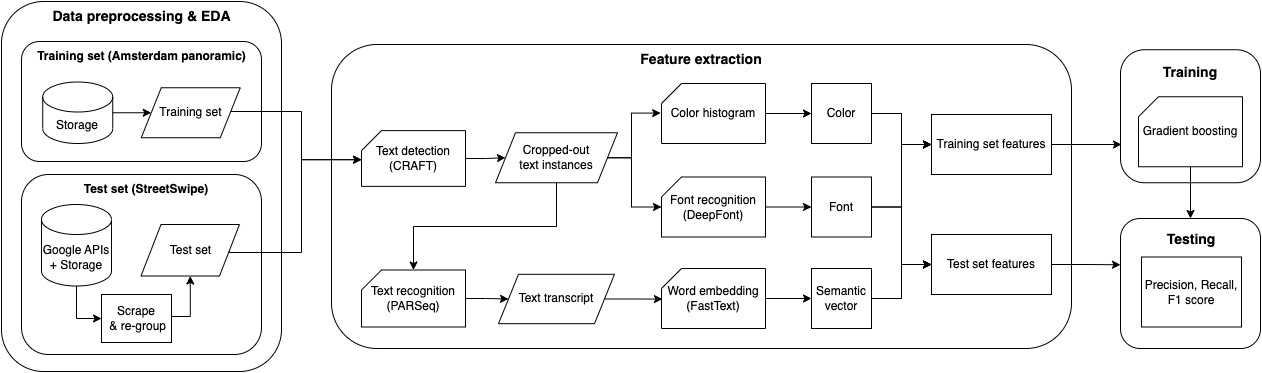
\includegraphics[width=\textwidth]{media/methodology/Pipeline.jpg}
    \caption{Pipeline: Images of facades labelled gentrified or non-gentrified are first fed into the text detection model to extract text instances. Subsequently, the text fonts are extracted with the font classifier, and color histograms are made to record the colors present in each text instances. Text strings are extracted with the text recognition model, before being converted into a vector embedding. Gradient boosting is trained and tested on these 3 features, to classify gentrified facades.}
    \label{fig:pipeline}
\end{figure*}

\subsection{Data}
\subsubsection{StreetSwipe}
The dataset with gentrified and non-gentrified labels is retrieved from the StreetSwipe project \cite{streetswipe}. Using crowd-sourcing, the project lets people decide whether each Amsterdam facade is gentrified, by voting "Yes" (gentrified) or "No" (non-gentrified) on the street view images of these facades. The official \textit{Gentrified} and \textit{Non-gentrified} labels for each facade are based on what the majority voted for. Additionally, if subsequent voters decide against the majority (e.g. voting \textit{Gentrified} for a non-gentrified-labelled facade), they are also prompted to provide a textual reasoning for their decision. These mismatch responses are also available, however is out of scope of the study. 

Since there are two versions of StreetSwipe, the data retrieved exists in two sets, consisting of 1912 higher resolution images from the older version and 529 lower resolution images from the new one. The StreetSwipe dataset thus have 2,441 images in total, each with its numbers of "Yes" and "No" votes, and metadata on the facade's location (latitude and longitude) and street name. The new version's images also have more detailed address, name, and type of business/services. There are also more votes in the new version than in the older version. The images from the old version are available directly, while the new ones were provided via URLs to a Google APIs bucket, and thus were scraped.

Feature engineering was done to create the gentrified/non-gentrified label per image, by taking the vote higher in volume. The images were then re-grouped per their corresponding label. Figure \ref{fig:class_size_SS} shows the sample size per class. There is class imbalance in the data, with more than 70\% of the images labelled non-gentrified. This is accounted for in evaluation by using appropriate metrics for classification performance.

\begin{figure}[H]
    \centering
    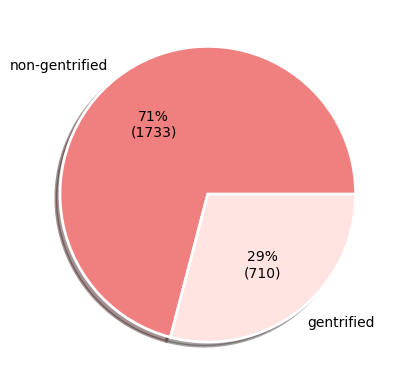
\includegraphics[width=0.4\textwidth]{media/methodology/SS_class_size.png}
    \caption{Sample size per class in StreetSwipe.}
    \label{fig:SS_class_size}
\end{figure}

\begin{figure}[H]
    \centering
    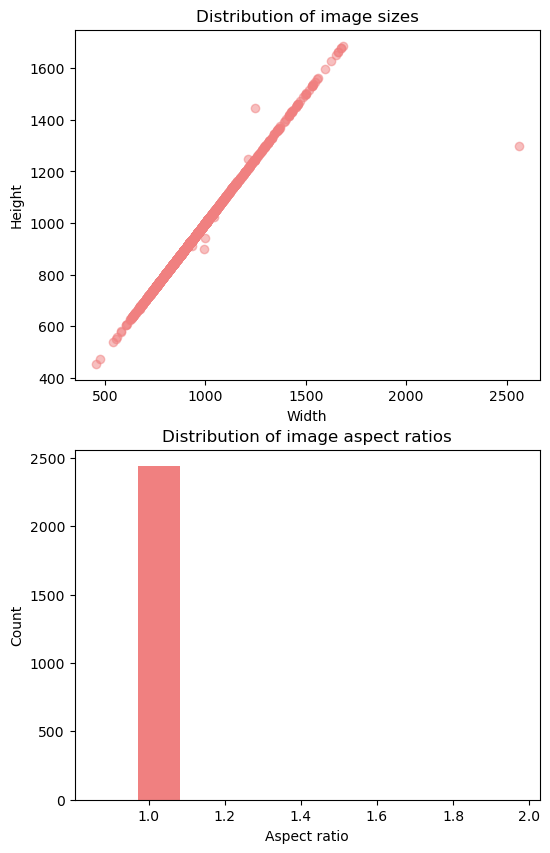
\includegraphics[width=0.35\textwidth]{media/methodology/SS_size_ar.png}
    \caption{Image sizes and aspect ratio distribution in StreetSwipe.}
    \label{fig:SS_size_ar}
\end{figure}

Figure \ref{fig:SS_size_ar} shows that the images have quite consistent aspect ratios of approximately 1:1; however, they vary in size, ranging from around 300x300 to 1700x1700, with one outlier of size approximately 2500x1300.

While this dataset contains valuable information - that is crowd-sourced label on gentrification - its size is sub-optimal for training a machine learning model. Therefore, it is used as the test set for the classifier, and another, larger data is used for training.

\subsubsection{Amsterdam panoramic street view data}
This data consists of panoramic street view images of 5 neighborhoods in Amsterdam: Amsterdamse Poort, Gaasperdam-Zuid, Elandsgrachtbuurt, Bellamybuurt-Noord, and Bellamybuurt-Zuid. This selection of neighborhoods represents gentrified and non-gentrified areas of the cities, based on existing urban studies literature. While Elandsgrachtbuurt (Jordaan) \cite{verlaan_hippies_2022}, Bellamybuurt-Noord, and Bellamybuurt-Zuid (Oud-West) \cite{rettberg_when_2019} have been identified as gentrified, Amsterdamse Poort and Gaasperdam-Zuid (Zuidoost) \cite{pinkster_stickiness_2020} are the opposite. Images of facades in these areas are thus labelled accordingly.

The images were provided with front, back, left, and right views of the vehicle already extracted. Out of these directions, facades appear most consistently on the left and right of the vehicles, therefore only these images are used in the study. All images have size 512x512.

(At the time of writing this draft section, the data was still being processed, due to its large volume. The current information is based on a subset already available; a more detailed and comprehensive exploratory data analysis on this dataset is still to be conducted.)

\subsection{Experimental setup}
\subsubsection{Scene-text detection - CRAFT}
The first task is to detect texts in the images of both the training and test sets, using CRAFT (Character-Region Awareness For Text detection) \cite{baek_character_2019} - a multi-lingual text detection model that is robust on curved and long texts.

The pre-trained model is applied on the data via the EasyOCR Python module \cite{noauthor_jaided_nodate}. More specifically, the \textit{detect} method was used, with text confidence threshold \textit{(text\_threshold)} set to 0.75, bounding box extension \textit{(add\_margin)} set to 0, and all other parameters set to their default values. This setting returns 2819 text instances in the images of the gentrified class, and 7680 in the non-gentrified class of the test set (work is still to be done for the training set). Text instances are cropped out by their bounding boxes and grouped per image, per class. 

\subsubsection{Color detection}
Color histograms \cite{srivastava_review_2015} will be made per text instance to extract the color feature. Through representing the text boxes as the frequency distribution of their colors, the text color can be identified as the most dominant color.

\subsubsection{Typeface recognition - DeepFont}
For recognizing the font type of the text, it is aimed that DeepFont \cite{wang_deepfont_2015} will be used. While the official model was not made available by the author, an implementation by \cite{reni_font_2023} can be trained on the AdobeVFR dataset \cite{wang_deepfont_2015} (as no pre-trained weights is available) and subsequently used to extract the font feature from the text boxes.

It can happen that this re-implementation does not return results of high enough quality. In such case, the font feature will be excluded from further analysis. This is due to both the limited time in the current research as well as a lack of existing resources in font recognition, especially for scene-text, and thus a lack of alternatives.

\subsubsection{Scene-text recognition - PARSeq}
To transcribe the image-text into machine-readable text strings, PARSeq \cite{bautista_scene_2022} will be used. Pre-trained model is available via Torch Hub. Subsequent to text recognition, certain strings will be excluded, such as "Google 2019" (the watermark from Google street view images), "sale", "taxi", "P" (on parking signs)... Such strings are spotted during the text detection phase, and are not of interest for semantic analysis.

\subsubsection{Semantic analysis - FastText}
The last feature to be extracted is text semantic. Vector representations of the extracted texts will be created using FastText \cite{bojanowski_enriching_2017}, which can provide embeddings for out-of-vocabulary words - a factor to be expected in the context of storefront signage.

\subsubsection{Classifier - Gradient boosting}
The features - color, font, semantic - of the training set will be used to train a gradient boosting classifier, with regards to whether a text instance is gentrified or not. Subsequently the model will be tested with the test set features.

\subsection{Evaluation}
Performance metrics - namely precision, recall, and F1 score - will be calculated for the classifier in validation and testing. The formulas are as follow:
\[Precision = \frac{True Positive}{True Positive + False Positive}\]

\[Recall = \frac{True Positive}{True Positive + False Negative}\]

\[F1 Score = \frac{2 * Precision * Recall}{Precision + Recall}\]
